\chptr{Relatività del Moto}
\marginpar{\minitoc}

\epigraph{\emph{``That view of things would be normal for me if I normally walked on my hands.''}}{\href{https://youtu.be/bJMYoj4hHqU?feature=shared&t=17}{\textcolor{blue}{\textit{Frames of Reference (1960) - Hume, Ivey}}}}

Ciò di cui si tratta in questo capitolo
è stato uno dei temi più controversi nella storia della fisica, quello
che forse ha sconvolto di più convinzioni un tempo ben radicate e
che ha infiammato dibattiti che hanno pure fatto la storia della
letteratura\footnote{\href{https://youtu.be/0kxarmulkiA?feature=shared&t=6180}{\textcolor{blue}{\textit{Marco Paolini - ITIS Galileo}}}.}. E non è tutto qui: Gli ultimi grandi sviluppi della relatività
del moto sono avvenuti poco più di un secolo fa ad opera di Einstein
e molti altri e i cambiamenti da loro apportati hanno condotto a
stravolgimenti ancora più bizzarri. Perché ciò che questo ramo della
fisica rivela è che più osserviamo con attenzione la realtà, più essa non
è come un attimo prima poteva sembrare. Per tale motivo la relatività può
essere allo stesso tempo semplice e complessa, perché offre una visione
del tutto insolita di ciò che ci appare come ``normale''.


\section{Sistemi di riferimento}
``Relativo'' è un termine che ben si sposa con l'espressione ``a qualcosa''.
Quel qualcosa viene definito nelle teorie relativistiche della fisica
\textit{sistema di riferimento}, che intuitivamente rappresenta il punto di
vista dal quale si effettuano delle misurazioni o semplici osservazioni di
fenomeni. Ricordiamo che tra le coordinate di un sistema di riferimento
è presente anche il tempo.

\begin{tcolorbox}[colback = yellow!30, colframe = yellow!30!black, title = {Sistema di riferimento}]
    Un insieme di strumenti geometrico-algebrici, di coordinate solidali con un
    oggetto arbitrario, e di procedure che consentono di individuare la posizione
    di un punto di uno spazio metrico.
\end{tcolorbox}

Una volta fissato il sistema di riferimento, tutte le misurazioni devono
essere coerenti con esso, se si intende adottare quel punto di vista.
Quando diciamo che un'auto viaggia a 110 km/h, stiamo in realtà fornendo
un'informazione incompleta, perché sottintendiamo che tale misurazione
sia stata effettuata rispetto alla strada. Non potremmo dire la stessa
cosa se viaggiassimo su un'altra auto che affianca la prima, con stessa
direzione e verso: Diremmo che
l'auto che prima, vista dalla strada, si muoveva a 110 km/h ora sta viaggiando con velocità
minore rispetto a noi. Il moto di un corpo è sempre relativo a un sistema di riferimento.
Cambiando il sistema, il moto cambia. Vedremo nei prossimi paragrafi
che però non tutti i sistemi di riferimento sono uguali e possono
distinguersi in \textit{inerziali} e \textit{non inerziali}.

Il cambiamento riguarda anche le traiettorie: Se lanciassimo una pallina
verso l'alto mentre viaggiamo sulla carrozza di un treno con velocità
costante, vedremmo la pallina salire e scendere su una linea retta.
Un osservatore esterno, invece vedrebbe la pallina muoversi secondo
una traiettoria parabolica. Vedremo che i moti si compongono
ed è necessario effettuare trasformazioni tra le coordinate dei
sistemi di riferimento.


\section{Principio di relatività galileiana}
In questo corso ci limitiamo a studiare sistemi di riferimento che
descrivono punti materiali che traslano e non ruotano in
alcun modo. Dato che molti oggetti sono in movimento l'uno rispetto
all'altro, vogliamo ora descrivere come essi sono tra loro legati,
ovvero come possiamo ``passare'' da un sistema all'altro, trasformando
le misure effettuate in un sistema in quelle che misureremmo nell'altro.

Supponiamo di avere due sistemi di riferimento, $S$ ed $S'$
centrati rispettivamente in $o$ e $o'$, come mostrati in figura
\ref{sistemi}. Consideriamo poi un punto materiale $P$ qualsiasi
e i vettori posizione che individuano $P$ nei rispettivi sistemi di riferimento:
otteniamo $\vecsymb{r}$, che è la posizione che $S$ misura,
e $\vecsymb{r}'$, misurata invece da $S'$. Ovviamente $S$ e $S'$
devono mettersi d'accordo su quale unità di misura impiegare, per
esempio il metro. Possiamo notare poi che il
sistema $S$ può misurare la posizione del centro $o'$ individuando
il vettore $\vecsymb{oo}'$. Ora è chiaro come questi vettori sono
in relazione:

\begin{align}
    \vecsymb{r} = \vecsymb{r}' + \vecsymb{oo}'\label{relpos}
\end{align}


\begin{marginfigure}
    \centering
    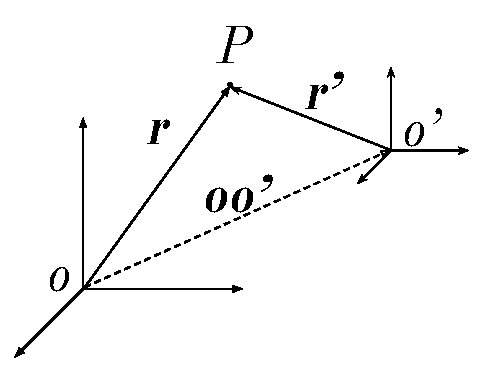
\includegraphics[width = \marginparwidth]{sistemi_relativi.pdf}
    \caption{Relazione tra due sistemi di riferimento che misurano
    la posizione del punto $P$.}
    \label{sistemi}
\end{marginfigure}

\noindent Non abbiamo fatto supposizioni sul moto relativo dei
due sistemi, ma se volessimo estendere l'analisi a velocità e
accelerazione di $P$ rispetto ai due sistemi è sufficiente
applicare alla \ref{relpos} le definizioni di velocità e accelerazione,
come visto in cinematica, derivando l'equazione:

\begin{align}
    \vecsymb{v} = \vecsymb{v}' + \vecsymb{v}_{o'}\\
    \vecsymb{a} = \vecsymb{a}' + \vecsymb{a}_{o'}
\end{align}

\noindent Notiamo che in queste equazioni compaiono $\vecsymb{v}_{o'}$
e $\vecsymb{a}_{o'}$, che corrispondono alla velocità e all'accelerazione
di $S'$ misurate in $S$. Se $\vecsymb{v}_{o'}$ non è nullo, allora
si può concludere che $S'$ si sta muovendo rispetto a $S$. Se $\vecsymb{a}_{o'}$
non è nullo, $S'$ sta accelerando rispetto ad $S$. Ci occuperemo nel seguito del
caso in cui $S$ è inerziale e $\vecsymb{a}_{o'}$ è nullo.

Dal momento che $S$ è inerziale, in esso vale la seconda legge della
dinamica $\vecsymb{F} = m\vecsymb{a}$. Essa avrà la stessa forma anche
in $S'$, che si muove rispetto a $S$ con $\vecsymb{v}_{o'}$ costante?
Ovvero, se $\vecsymb{F}$ è la forza in $S$ e $\vecsymb{F}' = m\vecsymb{a}'$ in $S'$,
varrà $\vecsymb{F} = \vecsymb{F}'$?
Dalle relazioni precedenti, possiamo notare che

\[ \vecsymb{F} = m\vecsymb{a} = m(\vecsymb{a}' + \vecsymb{a}_{o'}) = m\vecsymb{a}' + \frac{d}{dt}\vecsymb{v}_{o'} = m\vecsymb{a}' = \vecsymb{F}' \]

\noindent La seconda legge non è cambiata e possiamo dunque concludere
che $S'$ è un \textit{sistema di riferimento inerziale}.

\begin{tcolorbox}[colback = yellow!30, colframe = yellow!30!black, title = {Principio dei relatività galileiana}]
Le leggi della dinamica newtoniana hanno la stessa forma in tutti i
sistemi di riferimento inerziali.

Con riferimento alle proprietà cinematiche di posizione e velocità di
un punto materiale, il legame tra un sistema di riferimento inerziale,
con origine $o$, e un altro sistema di riferimento inerziale, con
origine $o'$, è descritta dalla seguente trasformazione:

\begin{align}
\begin{cases}
    \vecsymb{r} = \vecsymb{r}' + \vecsymb{oo}'\\
    \vecsymb{v} = \vecsymb{v}' + \vecsymb{v}_{o'}
\end{cases}
\end{align}
\end{tcolorbox}

\noindent In sistemi di riferimento inerziali, la velocità $\vecsymb{v}_{o'}$
prende il nome di \textit{velocità di trascinamento}.


\section{Forze apparenti}


\subsection{L'ascensore}
Per studiare meglio le forze apparenti, consideriamo il classico
esempio dell'ascensore. Quando ci troviamo in ascensore, nel
momento della partenza ci sentiamo più pesanti. Intuitivamente,
ciò accade per via dell'accelerazione della cabina diretta verso
l'alto, che ci preme sotto i piedi. Se invece l'ascensore comincia
a scendere, ci sentiamo invece più leggeri. Notare che ciò accade
solamente quando l'ascensore accelera.

Consideriamo il caso della salita. Trovandoci all'interno dell'ascensore,
immaginiamo di vedere il mondo esterno durante l'accelerazione. Noteremo
che dal nostro punto di vista la cabina rimane ferma, mentre il resto del
mondo scende verso il basso con il modulo della stessa accelerazione
dell'ascensore.


\section{Approfondimenti}
Spesso è facile ingannare la nostra percezione del moto. Le modalità
possono spaziare da tecniche molto semplici a intere teorie, come
quella della relatività di Einstein.

\subsection{Come \textit{Virtual Insanity} è stato girato}
Per coloro che non la conoscessero, \textit{Virtual Insanity} è
una canzone del 1996 dei \textit{Jamiroquai}. Il video
musicale\footnote{\href{https://www.youtube.com/watch?v=4JkIs37a2JE}{\textcolor{blue}{\textit{Jamiroquai - Virtual Insanity} (Official Video)}}},
rilasciato nel settembre di quell'anno, mostra il frontman Jay Kay
mentre danza e canta allegramente in una stanza asettica che, tra
le altre cose, sembrerebbe avere un pavimento in grado di traslare
in qualsiasi direzione. Se vi stupisce il fatto che un intero
pavimento possa muoversi su distanze così lunghe, in realtà il
meccanismo col quale il set venne realizzato fu più semplice di
quel che potrebbe sembrare, perché venne sfruttato il principio
sul quale si basa questo intero capitolo: il moto è relativo.

\begin{marginfigure}
    \centering
    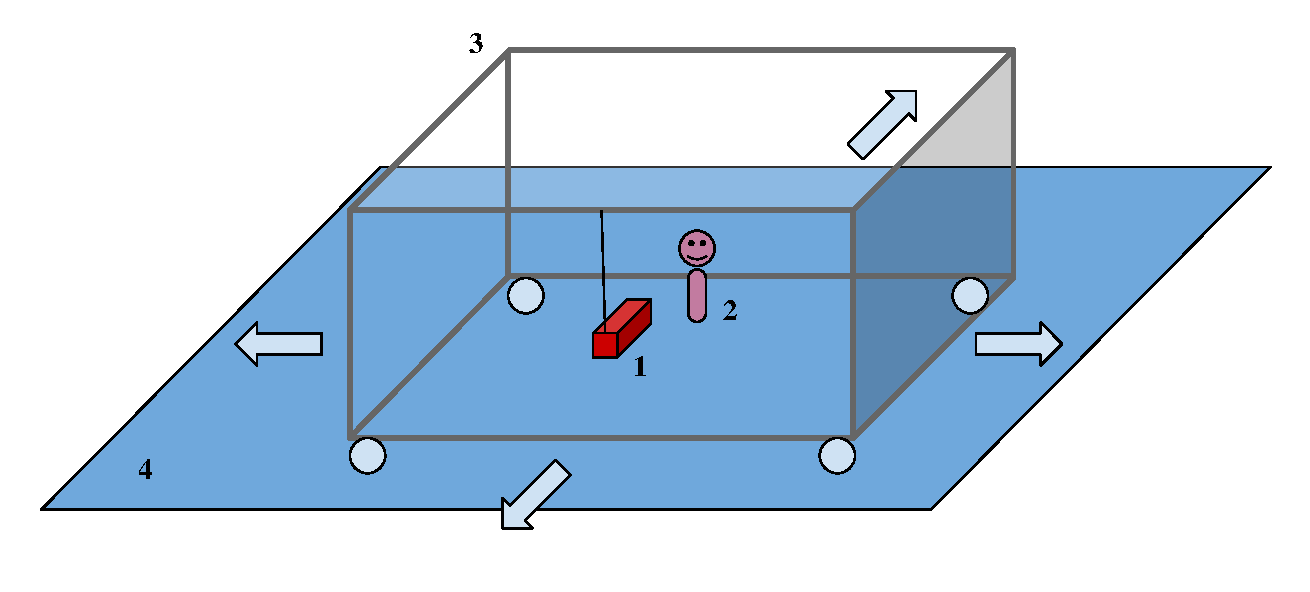
\includegraphics[width = \marginparwidth]{virtual_insanity.pdf}
    \caption{Schema semplificato del set realizzato per il video musicale:
    (1) telecamera fissata alla stanza mobile, (2) Jay Kay che si diverte,
    (3) stanza mobile, (4) pavimento del set.}
\end{marginfigure}


Secondo un'intervista rilasciata dal regista Jonathan Glazer\footnote{\href{https://www.youtube.com/watch?v=nY6YwZzKzTI}{\textcolor{blue}{Jamiroquai - The Story of Virtual Insanity
}}}, realizzare il video costruendo un pavimento mobile sarebbe
stato proibitivo, con costi nell'ordine delle centinaia di migliaia
di sterline. Fu così che, secondo quanto dichiarato, un membro del team di produzione
propose di muovere, invece del pavimento, l'intera stanza.
La telecamera sarebbe stata fissata all'impalcatura del set
(in fisica diremmo ``solidale con il sistema di riferimento
della stanza''), che sarebbe poi stato letteralmente mosso
su un ampio pavimento.
Qui, dunque, i sistemi di riferimento sono due: la stanza e il
pavimento. Tutti gli oggetti ``vivono'' nel proprio sistema
di riferimento per tutto il video, compresa la telecamera solidale
all'impalcatura, dando così l'impressione di
una stanza apparentemente ferma. Un caso interessante è
quello dei divani, che potevano essere fissati e agganciati
a piacimento alle pareti. Questo permetteva di trasferire
i mobili da un sistema di riferimento all'altro, dando un
tocco di mistero in più all'illusione. Ovviamente il risultato finale
è anche merito di un lavoro di post produzione da non sottovalutare.



%\section{Approfondimento: RR}
%Questa sezione è interamente dedicata alla relatività ristretta, sviluppata
%nelle sue forme più celebri da Einstein nei primi lustri del Ventesimo secolo.
%Vogliamo dare un assaggio di questa teoria per vari motivi: Si tratta in primo
%luogo di fisica classica (gli strumenti matematici impiegati sono pressoché gli stessi); essa è inoltre un buon esempio di ridefinizione e affinamento
%radicali di teorie precedenti, innanzitutto la relatività galileiana, e convinzioni
%comuni.

%\subsection{I principi della relatività ristretta}